\documentclass[a4paper,leqno,12pt]{amsart}
\usepackage{amssymb,amsthm,amsmath}
\usepackage[colorlinks,breaklinks]{hyperref}
\usepackage{tikz}
\usepackage{pgfplots}
\pgfplotsset{compat=1.11}
\usepgfplotslibrary{fillbetween}
\usetikzlibrary{intersections}
\usetikzlibrary{positioning,arrows}
\usetikzlibrary{shapes}
\usetikzlibrary{plotmarks}
\tikzset{
  state/.style={circle,draw,minimum size=6ex},
  arrow/.style={-latex, shorten >=1ex, shorten <=1ex}}
\usetikzlibrary{patterns}

\begin{document}

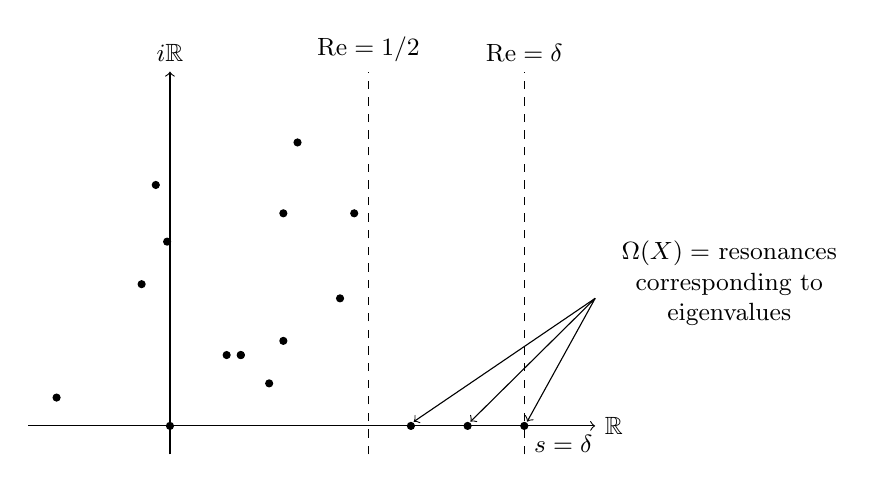
\begin{tikzpicture}[xscale=1.8, yscale=1.8]
%real axis
    \draw [->] (-1,0) -- (3,0) node [right, font=\small]  {$  \mathbb{R} $};
%imaginary axis
    \draw [->] (0,-0.2) -- (0,2.5) node [above, font=\small] {$ i \mathbb{R} $};
%delta-axis        
    \draw[dashed] (2.5,-0.2) -- (2.5,2.5) node [above, font=\small] {$ \mathrm{Re}= \delta $};
%1/2-axis
	\draw[dashed] (1.4,-0.2) -- (1.4,2.5) node [above, font=\small] {$ \mathrm{Re} = 1/2 $};
%delta
    \filldraw (2.5,0) circle (0.7pt) node[below right, font=\small] {$s=\delta$};
%some eigenvalues
    \filldraw (1.7,0) circle (0.7pt);
    \filldraw (2.1,0) circle (0.7pt);
% resonance at origin
	\filldraw (0,0) circle (0.7pt);
% other resonances
	\filldraw (0.8,0.6) circle (0.7pt);
	\filldraw (0.4,0.5) circle (0.7pt);
	\filldraw (0.7,0.3) circle (0.7pt);
	\filldraw (-0.2,1) circle (0.7pt);
	\filldraw (-0.8,0.2) circle (0.7pt);
	\filldraw (0.9,2) circle (0.7pt);
	\filldraw (-0.1,1.7) circle (0.7pt);
	\filldraw (0.8,1.5) circle (0.7pt);
	\filldraw (-0.02,1.3) circle (0.7pt);
	\filldraw (0.5,0.5) circle (0.7pt);
	\filldraw (1.3,1.5) circle (0.7pt);
	\filldraw (1.2,0.9) circle (0.7pt);
	\filldraw (0.5,0.5) circle (0.7pt);
%labeling eigenvalues
   	\draw (3,1) node[right, font=\small] {\begin{tabular}{c}
    $\Omega(X) =$ resonances \\
    corresponding to \\ 
    eigenvalues
\end{tabular}};
	\draw[->] (3,0.9) -- (2.52,0.03);
   	\draw[->] (3,0.9) -- (1.72,0.03);
   	\draw[->] (3,0.9) -- (2.12,0.03);
%labeling other resonances
\end{tikzpicture}

\end{document}